
==============================

The end (below is the copy-paste from IJCAI paper) The end

==============================



% START COPY AND PASTE FROM WORKSHOP PAPER

% Setting: we took grid-based setting
We conducted experiments on grids, where agents can move from the center of one grid cell 
to the center of another grid cell. 
The size of every cell is $1\times 1$, and 
the shape of every agent is a an open disk which radius equals $\sqrt{2}/4$. This specific value was chosen to allow comparison with \cbs, since it is the maximal radius that allows agents to safely perform moves in which agents follow each other.
%\footnote{In particular, this is the largest agent radius that allows the following pair of actions: agent $i$ goes up from cell $X$ to cell $Y$, and at the same time agent $j$ moves to $X$ from the right. While such train-like movements are not allowed by some \ac{MAPF} variants, they are assumed to be valid in most in research on \cbs.}




% The 2^k neighborhood
To allow non-unit edge costs, we allowed agents to move in a single move action to every cell located in their $2^k$ neighborhood, where $k$ is a parameter~\cite{rivera2017grid}. Moving from one cell to the other is only allowed if the agent can move safely to the goal cell without colliding with other agents or obstacles, where the geometry of the agents and obstacles are considered. The cost of a move corresponds to the Euclidean distance between the grid cells centers.  Figure~\ref{fig:2k} illustrates such a $2^k$ neighborhood. Increasing $k$ means a search space with higher branching factor, but also allows finding lower cost plans. 
%\roni{Maybe this is vague?} 
%As a heuristics, we pre-computed the all-pairs shortest-path distance between every pair of locations in the map, which is a perfect heuristic for single agent search. \roni{Removed for space constraints}


\subsection{Open Grids}
% First setup: open 10x10 grids, varying values of $k$
% Please add the following required packages to your document preamble:
% \usepackage{booktabs}
\begin{table}
\centering
\resizebox{0.8\columnwidth}{!}{
\begin{tabular}{@{}c|cccc|cccc@{}}
\toprule
   & \multicolumn{4}{|c}{\ac{SOC}}   & \multicolumn{4}{|c}{Success Rate} \\ \midrule
$k$ & 2     & 3    & 4    & 5    & 2    & 3    & 4    & 5    \\ \midrule
4      & 25.7  & 21.2 & 20.4 & 20.3 & 1.00 & 1.00 & 0.97 & 0.95 \\
%5      & 31.7  & 26.2 & 25.3 & 25.1 & 0.99 & 1.00 & 0.92 & 0.90 \\
6      & 38.2  & 31.6 & 30.5 & 30.2 & 0.99 & 1.00 & 0.88 & 0.83 \\
%7      & 43.8  & 36.2 & 35.0 & 34.7 & 0.98 & 0.98 & 0.84 & 0.70 \\
8      & 49.2  & 40.7 & 39.3 & 39.0 & 0.98 & 0.97 & 0.74 & 0.57 \\
%9      & 55.0  & 45.5 & 43.9 & 43.5 & 0.98 & 0.97 & 0.61 & 0.50 \\
10     & 61.0  & 50.5 & 48.8 & 48.4 & 0.95 & 0.94 & 0.54 & 0.42 \\
%11     & 68.7  & 56.8 & 54.9 & -  & 0.95 & 0.88 & 0.43 & - \\
12     & 78.0  & 64.7 & -  & -  & 0.94 & 0.86 & - & - \\
%13     & 84.6  & 70.2 & -  & -  & 0.92 & 0.76 & - & - \\
14     & 90.8  & 75.3 & -  & -  & 0.88 & 0.64 & - & -  \\
%15     & 97.1  & 80.7 & -  & -  & 0.82 & 0.58 & -  & -  \\
16     & 102.4 & 85.2 & -  & -  & 0.76 & 0.53 & -  & -  \\
%17     & 108.3 & 90.4 & -  & -  & 0.71 & 0.42 & -  & -  \\
18     & 118.7 & -  & -  & -  & 0.62 & - & -  & -  \\
%19     & 125.5 & -  & -  & -  & 0.56 & -  & -  & -  \\
20     & 131.7 & -  & -  & -  & 0.46 & -  & -  & - \\\bottomrule
\end{tabular}
}
\caption{Results for \ccbs on $10\times 10$ open grid.}% for $k=2, 3, 4$, and $5$}
\label{tab:10x10}
\vspace{-0.3cm}
\end{table}

\commentout{
\begin{table}
\resizebox{\columnwidth}{!}{
\begin{tabular}{@{}c|cccc|cccc@{}}
\toprule
   & \multicolumn{4}{|c}{\ac{SOC}}   & \multicolumn{4}{|c}{Success Rate} \\ \midrule
$k$ & 2     & 3    & 4    & 5    & 2    & 3    & 4    & 5    \\ \midrule
4      & 25.7  & 21.2 & 20.4 & 20.3 & 1.00 & 1.00 & 0.97 & 0.95 \\
5      & 31.7  & 26.2 & 25.3 & 25.1 & 0.99 & 1.00 & 0.92 & 0.90 \\
6      & 38.2  & 31.6 & 30.5 & 30.2 & 0.99 & 1.00 & 0.88 & 0.83 \\
7      & 43.8  & 36.2 & 35.0 & 34.7 & 0.98 & 0.98 & 0.84 & 0.70 \\
8      & 49.2  & 40.7 & 39.3 & 39.0 & 0.98 & 0.97 & 0.74 & 0.57 \\
9      & 55.0  & 45.5 & 43.9 & 43.5 & 0.98 & 0.97 & 0.61 & 0.50 \\
10     & 61.0  & 50.5 & 48.8 & 48.4 & 0.95 & 0.94 & 0.54 & 0.42 \\
11     & 68.7  & 56.8 & 54.9 & -  & 0.95 & 0.88 & 0.43 & 0.31 \\
12     & 78.0  & 64.7 & -  & -  & 0.94 & 0.86 & 0.32 & 0.24 \\
13     & 84.6  & 70.2 & -  & -  & 0.92 & 0.76 & 0.22 & 0.15 \\
14     & 90.8  & 75.3 & -  & -  & 0.88 & 0.64 & 0.18 & -  \\
15     & 97.1  & 80.7 & -  & -  & 0.82 & 0.58 & -  & -  \\
16     & 102.4 & 85.2 & -  & -  & 0.76 & 0.53 & -  & -  \\
17     & 108.3 & 90.4 & -  & -  & 0.71 & 0.42 & -  & -  \\
18     & 118.7 & -  & -  & -  & 0.62 & 0.32 & -  & -  \\
19     & 125.5 & -  & -  & -  & 0.56 & -  & -  & -  \\
20     & 131.7 & -  & -  & -  & 0.46 & -  & -  & - \\\bottomrule
\end{tabular}
}
\caption{Results for \ccbs on $10\times 10$ open grid.}% for $k=2, 3, 4$, and $5$}
\label{tab:10x10}
\end{table}
}

For the first set of experiments we used a
$10\times 10$ open grid, placing agents' start and goal locations randomly. We run experiments with 4, 5, $\ldots, 20$ agents. For every number of agents we created 250 different problems. 
Each problem was solved with \ccbs with $k=2, 3, 4$, and $5$. 
%\roni{TODO: Add supp.} 
An animation of a solution found by \ccbs for a problem with 13 agents and different values of $k$ can be seen in \url{https://tinyurl.com/ccbs-example}.
%The file \texttt{CCBS.mp4} in the supplementary material shows an animation of the solution found by \ccbs for a problem with 13 agents and different values of $k$. 
Table~\ref{tab:10x10} shows the results of this set of experiments. 
 Every row shows results for a different number of agents, 
as indicated on the left-most column. 
The four right-most columns show the success rate, i.e., the ratio of problems solved by the \ccbs under a timeout of 60 %\roni{Anton what was the timeout?} 
seconds, out of a total of 250 problems. 
Data points marked by ``-'' indicate settings where the success rate was lower than 0.4. The next four columns show the average \ac{SOC}, 
averaged over the problems solved by all \ccbs instances that had a success rate larger than 0.4. 

%\roni{Was this the cutoff?} \textbf{K: Actually the cut-off was "lower than 50\%", but Anton continued running the experiments when it was not super time-consuming. That is why we have some extra data points.}

The results show that increasing $k$ yields solutions with lower \ac{SOC}, as expected. 
The absolute difference in \ac{SOC} when moving from $k=2$ to $k=3$ is the largest, and it grows as we add more agents. For example, for problems with 14 agents, moving from $k=2$ to $k=3$ yields an improvement of 15.5 \ac{SOC}, 
and for problems with 16 agents the gain of moving to $k=3$ is 17.2 \ac{SOC}. Increasing $k$ further exhibits a diminishing return effect, where the largest average \ac{SOC} gain when moving from $k=4$ to $k=5$ is at 0.5. 
%\roni{Maybe bla a bit on why this is, although I think it is obvious.} 



Increasing $k$, however, has also the effect of increasing the branching factor, which in turns means that path-finding becomes harder. Indeed, the success rate of $k=5$ is significantly lower compared to $k=4$. An exception to this is the transition from $k=2$ to $k=3$, where we observed a slight advantage in success rate for $k=3$ for problems with a small number of agents. For example, with 6 agents the success rate of $k=2$ is 0.99 while it is 1.00 for $k=3$. An explanation for this is that increasing $k$ also means that plans for each agent can be shorter, which helps to speedup the search. Thus, increasing $k$ introduces a tradeoff w.r.t. the problem-solving difficulty: the resulting search space for the low-level search is shallower but wider. For denser problems, i.e., with more agents, $k=2$ is again better in terms of success rate, as more involved plans must be found by the low-level search. 

\commentout{
\begin{figure}
    \centering
    \includegraphics[width=\columnwidth]{soc-gain.PNG}
    \caption{10$\times$10 open grid, gain of using \ccbs over  \cbs.}
    \label{fig:soc-gain}
\end{figure}
Figure~\ref{fig:soc-gain} shows the tradeoff of increasing $k$ by showing the average \emph{gain}, in terms of \ac{SOC}, of using \ccbs for different values of $k$
over \ccbs with $k=2$. The $x$-axis is the number of agents, and the $y$-axis is the gain, in percentage. We only provide data points for configurations with a success rate of at least 40\%. As can be seen, increasing $k$ increases the gain over \cbs, where for $k=4$ and $k=5$ the gain was over 20\%. Increasing $k$ also decreases the success rate, and thus the data series for larger $k$ value ``disappears'' after a smaller number of agents. 
}

1

%To see this phenomenon, consider the example in Figure~\ref{fig:anton-example}. There are three agents, 1,2, and 3 in an open 2$\times$4 grid.  The left-most grid shows the initial locations of the agents,  and the right-most grid shows their goal locations. The small arrows in the agents indicate the direction each agent is about to move to.  Consider first the plan created by \cbs, which is shown on the top row of Figure~\ref{fig:anton-example}. In \cbs,  every action takes unit duration. Since agent 3 cannot move upwards at time $t=0$ without colliding with agent 1, it will have to wait for time $t=1$ before starting to move.  By contrast, in \ccbs a wait action can have an arbitrary duration, and thus agent 3 can start to move upwards safely earlier than in \cbs, at time $t=0.707$. See the file \texttt{C-CBSvsCBS.gif} in the supplementary material for an animation of this example. These cases, where \ccbs with $k=2$ finds a better solution compared to standard \cbs, are not rare. However, the advantage in terms of \ac{SOC}, in all our experiments, was very small. 




\subsection{Dragon Age Maps}
%\begin{figure}
%    \centering
%    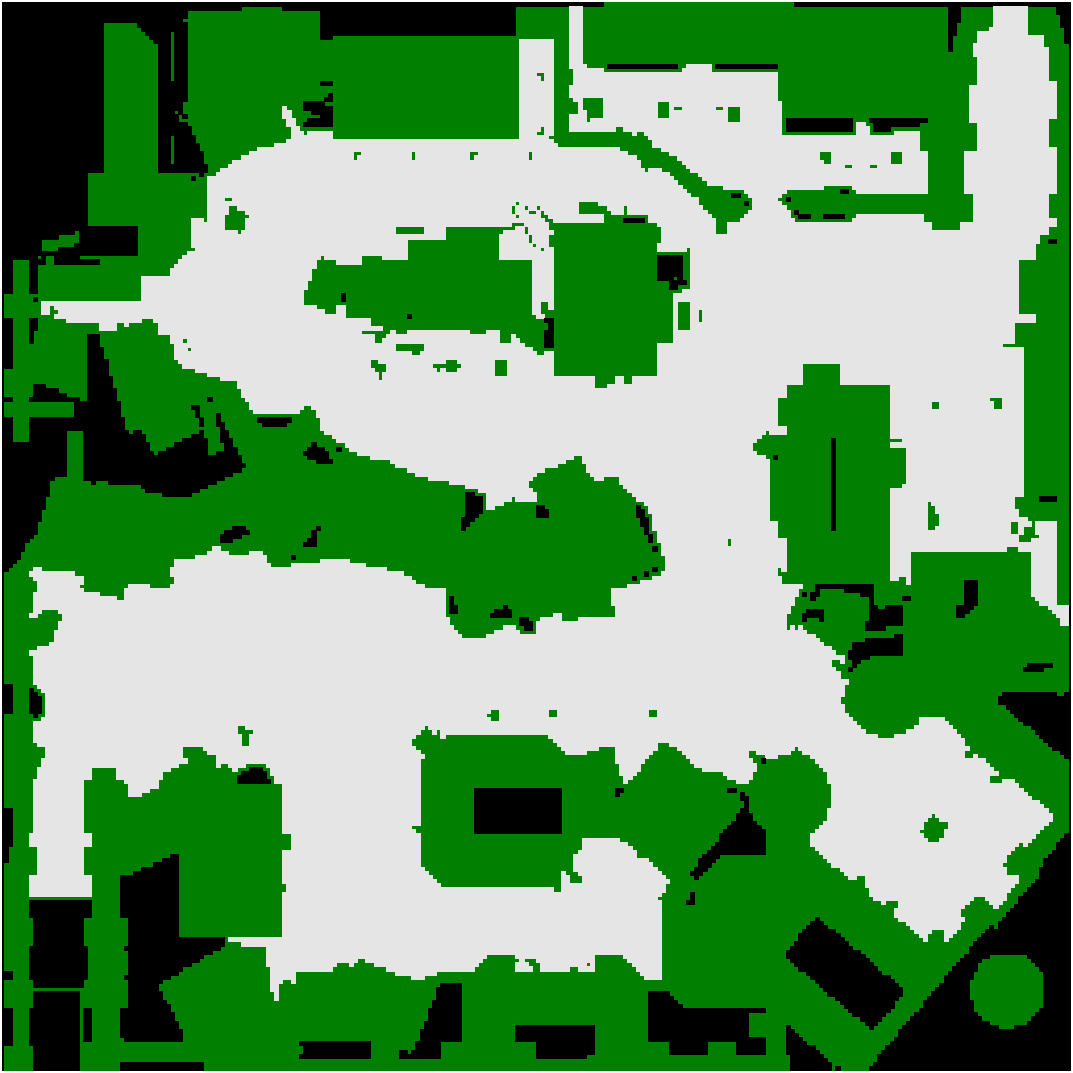
\includegraphics[width=0.5\columnwidth]{den520d.png}
%    \caption{The \texttt{den520d} DAO map used in our experiments. \roni{Add some more figures near by to save space.}}
%    \label{fig:dao}
%\end{figure}


% Please add the following required packages to your document preamble:
% \usepackage{booktabs}
\begin{table}
\centering
\resizebox{0.7\columnwidth}{!}{
    \begin{tabular}{@{}c|ccc|ccc@{}}
    \toprule
    \multicolumn{1}{l|}{} & \multicolumn{3}{c|}{\ac{SOC}} & \multicolumn{3}{c}{Success Rate} \\ \midrule
    k                     & 2      & 3      & 4      & 2         & 3         & 4        \\ \midrule
    10                    & 1,791  & 1,515  & 1,460  & 0.96      & 0.93      & 0.86     \\
    15                    & 2,598  & 2,198  & 2,118  & 0.94      & 0.84      & 0.70     \\
    20                    & 3,347  & 2,829  & 2,726  & 0.79      & 0.72      & 0.50     \\
    25                    & 4,049  & 3,426  & 3,304  & 0.58      & 0.58      & 0.32     \\ \bottomrule
    \end{tabular}
}
$\vcenter{\hbox{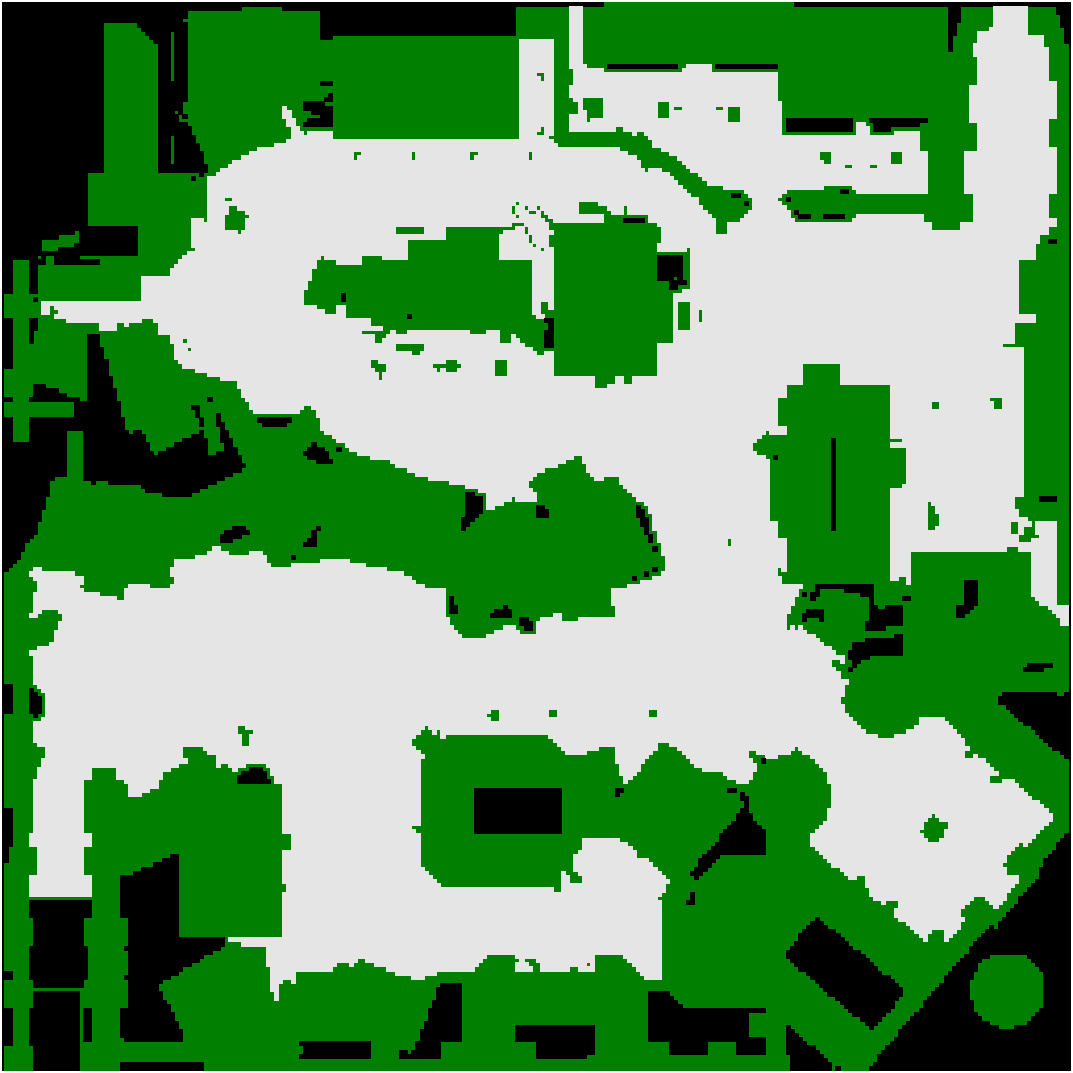
\includegraphics[width=0.25\columnwidth]{den520d.png}}}$
    %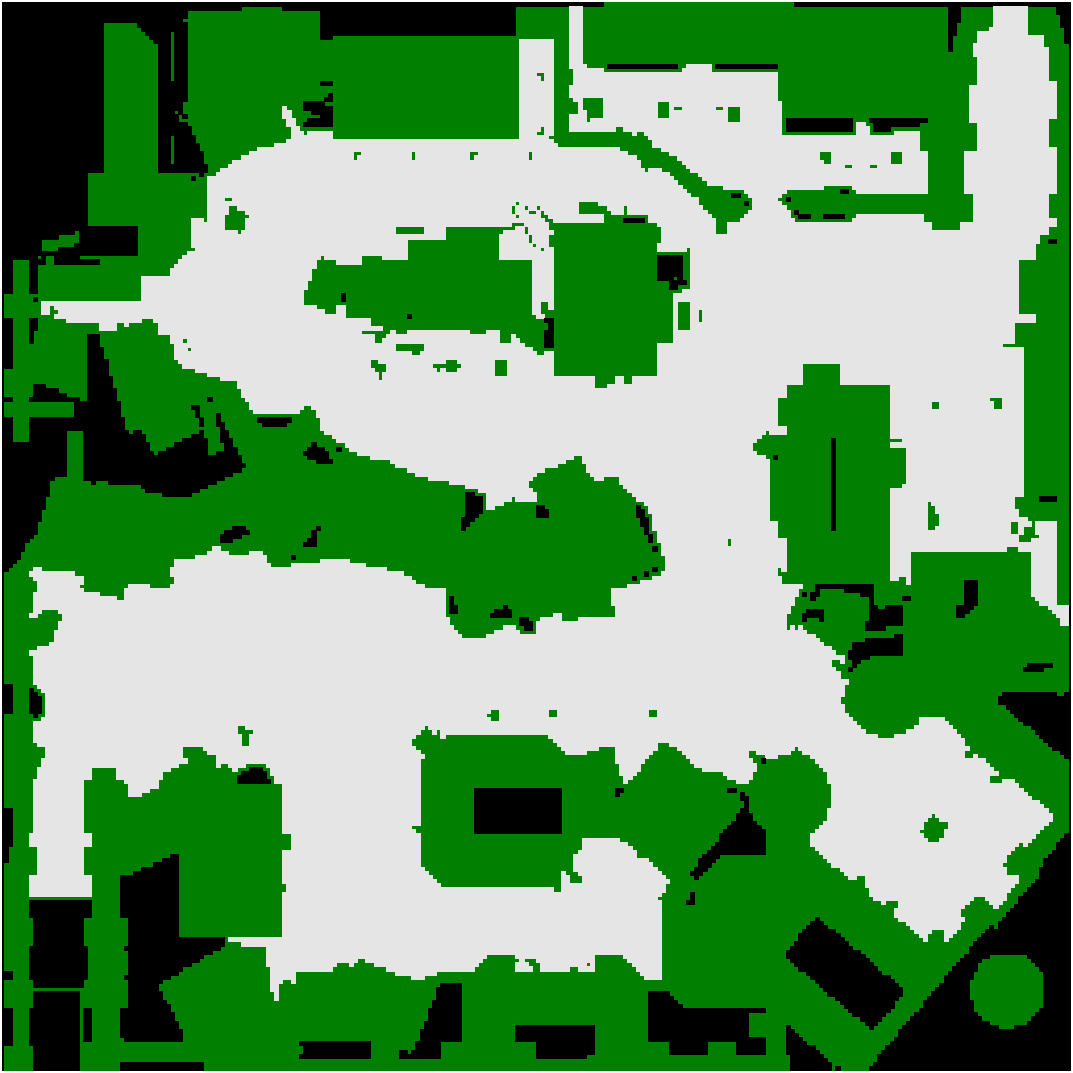
\includegraphics[width=0.25\columnwidth]{den520d.png}

\caption{Results for \ccbs on the \texttt{den520d} DAO map.}
\label{tab:dao}
\vspace{-0.3cm}
\end{table}

% Different k values DAO
Next, we experimented with a larger grid, taken from the Dragon Age: Origin (DAO) game and made available in the \texttt{movingai} repository~\cite{sturtevant2012benchmarks}. We used the \texttt{den520d} map, shown to the right of Table~\ref{tab:dao}, which was used by prior work~\cite{sharon2015conflict}. 
Start and goal states were chosen randomly, and we create 250 problems for every number of agents.
%\roni{Anton: did you choose start and goal randomly, or using some other method?}Anton: yes, randomly
\commentout{
\begin{figure}
    \centering
    \includegraphics[width=\columnwidth]{runtime-dao_cropped.pdf}
    \caption{The average runtime for the DAO map.}
    \label{fig:dao-runtime}
\end{figure}
}
Table~\ref{tab:dao} shows the results obtained for \ccbs with $k=2,3,$ and $4$, 
in the same format as Table~\ref{tab:10x10}. The same overall trends are observed: increasing $k$ reduces the SOC and decreases the success rate. %Figure~\ref{fig:dao-runtime} shows the  average runtime required to solve the instances solved by all values of $k$. Interestingly, here we observe that $k=3$ was the fastest on average. Similar to the better success rate in the open grid experiments, we explain this by the fact that increasing $k$ also yields shorter paths to the goals, which helps decrease runtime. %This behavior corresponds to the results reported in the previous set of experiments. observed for the open gri

%\roni{Maybe put here the roadmap experiments?}


\subsection{Conflict Detection and Resolution Heuristics}


% Please add the following required packages to your document preamble:
% \usepackage{booktabs}

\begin{table}
\centering
\resizebox{0.9\columnwidth}{!}
{
\begin{tabular}{@{}lrrrrr@{}}
\toprule
  & &\multicolumn{1}{c}{Vanilla} & \multicolumn{1}{c}{PastConf} & \multicolumn{1}{c}{Cardinals} & \multicolumn{1}{c}{Hybrid} \\ \midrule

%\multirow{3}{*}{\begin{sideways}20 agents\end{sideways}} & \multirow{3}{*}{\begin{sideways}$k$=2\end{sideways}} & Succ.     & 0.72   & 0.74 & 0.75 & 0.82\\
\multirow{2}{*}{
\parbox{1.5cm}{$k$=2 Agents=20}} & Success     & 0.72   & 0.74 & 0.75 & 0.82         \\
%& Time     & 4.57   & 3.55 & 5.86 & 2.16                      \\
& HL exp. & 765    & 712 & 453 & 452                    \\ \midrule
\multirow{2}{*}{\parbox{1.5cm}{$k$=3 Agents=20}} & Success     & 0.67   & 0.68    & 0.75      & 0.76   \\
%& Time     & 1.83   & 1.65    & 1.70      & 1.51   \\
& HL exp.  & 152    & 141     & 51        & 47     \\ \midrule
\multirow{2}{*}{\parbox{1.5cm}{$k$=4 Agents=20}} & Success     & 0.39   & 0.4    & 0.48      & 0.50   \\
%& Time     & 4.67   & 3.84    & 3.83      & 2.71   \\
& HL exp.  & 564    & 516     & 232       & 270     \\ \midrule
\multirow{2}{*}{\parbox{1.5cm}{$k$=2 Agents=25}} & Success  & 0.39   & 0.43    & 0.38      & 0.53   \\
%& Time     & 10.25  & 7.33   & 13.08    & 3.66  \\
& HL exp. & 1762   & 1730    & 968       & 990  \\ \midrule
\multirow{2}{*}{\parbox{1.5cm}{$k$=3 Agents=25}} & Success  & 0.44   & 0.45    & 0.60      & 0.61   \\
%& Time     & 3.32  & 2.74   & 2.88    & 2.34  \\
& HL exp. & 313   & 270   & 81       & 72  \\ \bottomrule

\end{tabular}
}
\caption{Comparing conflict detection and selection methods.}
\label{tab:heuristics}
\end{table}

%\multirow{-10}{*}{\cellcolor{yellow}\begin{sideways}TEST\end{sideways}}%

In all the experiments so far we have used \ccbs with the hybrid conflict detection and selection heuristic described earlier in the paper. Here, we evaluate the benefit of using this heuristic. We compared \ccbs with this heuristic against the following: (1) Vanilla: \ccbs that chooses arbitrarily which actions to check first for conflicts, 
(2) Cardinals: \ccbs that identifies all conflicts and chooses cardinal conflicts,   
and (3) PastConf: \ccbs that uses the \history heuristic to choose where to search for conflicts first, and resolves the first conflict it finds.  

%Table~\ref{tab:heuristics} shows results for experiments run on the \texttt{den520d} DAO map.
Table~\ref{tab:heuristics} shows results for the \texttt{den520d} DAO map for 20 agents with $k=$ 2, 3, and 4; and 25 agents with $k$=2 and $k$=3. For every configuration we create and run \ccbs on 1,000 instances. The table shows the success rate (the row labelled ``Success'')  
%the average runtime in seconds over instances solved by all algorithms (``Time''), 
and the average number of high-level nodes expanded by \ccbs (``HL exp.''). The results show that the proposed hybrid heuristic 
enjoys the complementary benefits of PastConf and Cardinals, 
expanding as few \ct nodes as Cardinals 
and having the highest success rate. %, expanding as few \ct nodes as Cardinals and enjoys the complementary benefits of PastConf and Cardinals: , as can be seen by its high success rate and small number of high-level expanded nodes. Thus, we used it in all our experiments. 

%When comparing PastConf to Cardinals, we see that PastConf has a higher success rate but the number of high-level nodes expanded by Cardinals is smaller. This follows our motivation for the hybrid heuristic: the choice of which conflicts to resolve taken by Cardinals is important in minimizing the size of the CT, while detecting all conflicts can be too time consuming. The proposed hybrid heuristic enjoys the complementary benefits of PastConf and Cardinals, as can be seen by its high success rate and small number of high-level expanded nodes. Thus, we used it in all our experiments. 
%its fast runtime and small number of high-level expanded nodes. Thus, we used it in all our experiments. 
  

\commentout{
\begin{figure}
    \centering
    \includegraphics[width=0.35\columnwidth]{roadmap_cropped.pdf}
    \caption{The roadmap created for \texttt{den520d} DAO map.}
    \label{fig:roadmap}
\end{figure}
}
We also performed a limited set of experiments on roadmaps, to demonstrate the applicability of \ccbs beyond grid domains. 
%We created roadmaps  based on the the \texttt{den520d} DAO map using the OMPL library (http://ompl.kavrakilab.org), which is a widely used robotics library for path planning.
%Figure~\ref{fig:roadmap} shows a roadmap 
We created a roadmap with 878 vertices and 14,628 edges based on the \texttt{den520d} DAO map using the OMPL library (http://ompl.kavrakilab.org). 
%, which is a widely used robotics library for path planning. 
We create 250 problems with 10, 15, and 20 agents. The resulting success rate was 0.89, 0.60, and 0.22, 
and the SOC was 1,459, 2,082, and 2,688, respectively. 
In \url{https://tinyurl.com/ccbs-roadmap2} there is an animation showing a solution found by \ccbs for a small roadmap. 

